\subsection{Funktionsnachweis kritischer Funktionen}
Dieses Unterkapitel befasst sich mit dem praktischen Nachweis von kritischen Teilfunktionen. Kritische Teilfunktionen sind Funktionen, welche bei einem Ausfall dieser Teilfunktion, einen Ausfall des Gesamtsystems zur Folge hat. Dabei soll die Umsetzung einfacher Funktionsmuster einen praktischen Nachweis bringen, ob die Umsetzung von dieser Teillösung realistisch ist. Diese Beurteilung wird für Bewertung der ausgearbeiteten Lösungskonzepte miteinbegezogen.
\newline
Bei Betrachtung der Funktionsanalysen (Abbildungen \ref{fig:FunktPflicht} und \ref{fig:FunktWunsch}) ist erkennbar, dass beide Varianten (Pflicht sowie Wunsch) eine Serieschaltung darstellen. Bei einer Umsetzung einer Maschine mit einfacher Redundanz ergibt dies implizit, dass jede Funktion als kritisch eingestuft werden kann. Aus zeitlichen Gründen kann ein umfassenden Nachweis von allen Teillösungskonzepten nicht abschliessend durchgeführt werden. Eine pragmatische Auswahl von Funktionen mit erhöhtem Ausfallrisiko und einer vielversprechenden Funktionserfüllung wird daher angestrebt.

\subsubsection{NemaCaps vereinzeln und fördern}
Die Vereinzelung sowie Förderung von Gütern ist in der Automatisationsbranche ein bedeutendes Thema. Die automatisierte Sortierung sowie Transport eines Gutes sind grundlegende Bedingungen, sodass ein Produkt überhaupt in der automatisierten Serienfertigung herstellbar wird. Da solche Lösungen vielfach beide Funktionen miteinander vereinen, werden diese gemeinsam in einem Unterkapitel untersucht.
\newline
\newline
\textbf{Vibrationswendelförderer}
\newline
Ein Gerät das die Verzeinzelung sowie Förderung von Werkstücken vereint ist der Vibrationswendelförderer. Mittels Schwingungsenergie wird eine Wanderbewegung der Werkstücke erzeugt, welche beim Passieren von Schikanen vereinzelt werden. Weitere Erklärungen zum Wendelförderer sind im \textbf{Anhang} zu entnehmen.
\newline
Aus vergangenen Studentenarbeiten besitzt die Hochschule Luzern für Technik und Architektur einen solchen Wendelförderer. Dimensioniert ist dieser für die Vereinzelung von gezuckerten Mandeln. Auch wenn dadurch die Vereinzelung nur bedingt funktionsfähig ist, eignet sich dieses Gerät zur ersten Überprüfung der Funktion mit NemaCaps. 

Praktische Tests mit NemaCaps konnten am 15.3.2017 am Wendelförderer durchgeführt werden. NemaCaps wurden ins Haufwerk (Punkt 1 in Abbildung \ref{fig:wendelfoerderer}) eingefüllt und der Wendelförderer gestartet. Durch die Vibration sammelten sich die NemaCaps im Wendel (2) und begannen zu wandern. Die Förderung klappte einwandfrei, wobei die rasche Transportgeschwindigkeit positiv überraschte. 
\begin{figure}[H]
	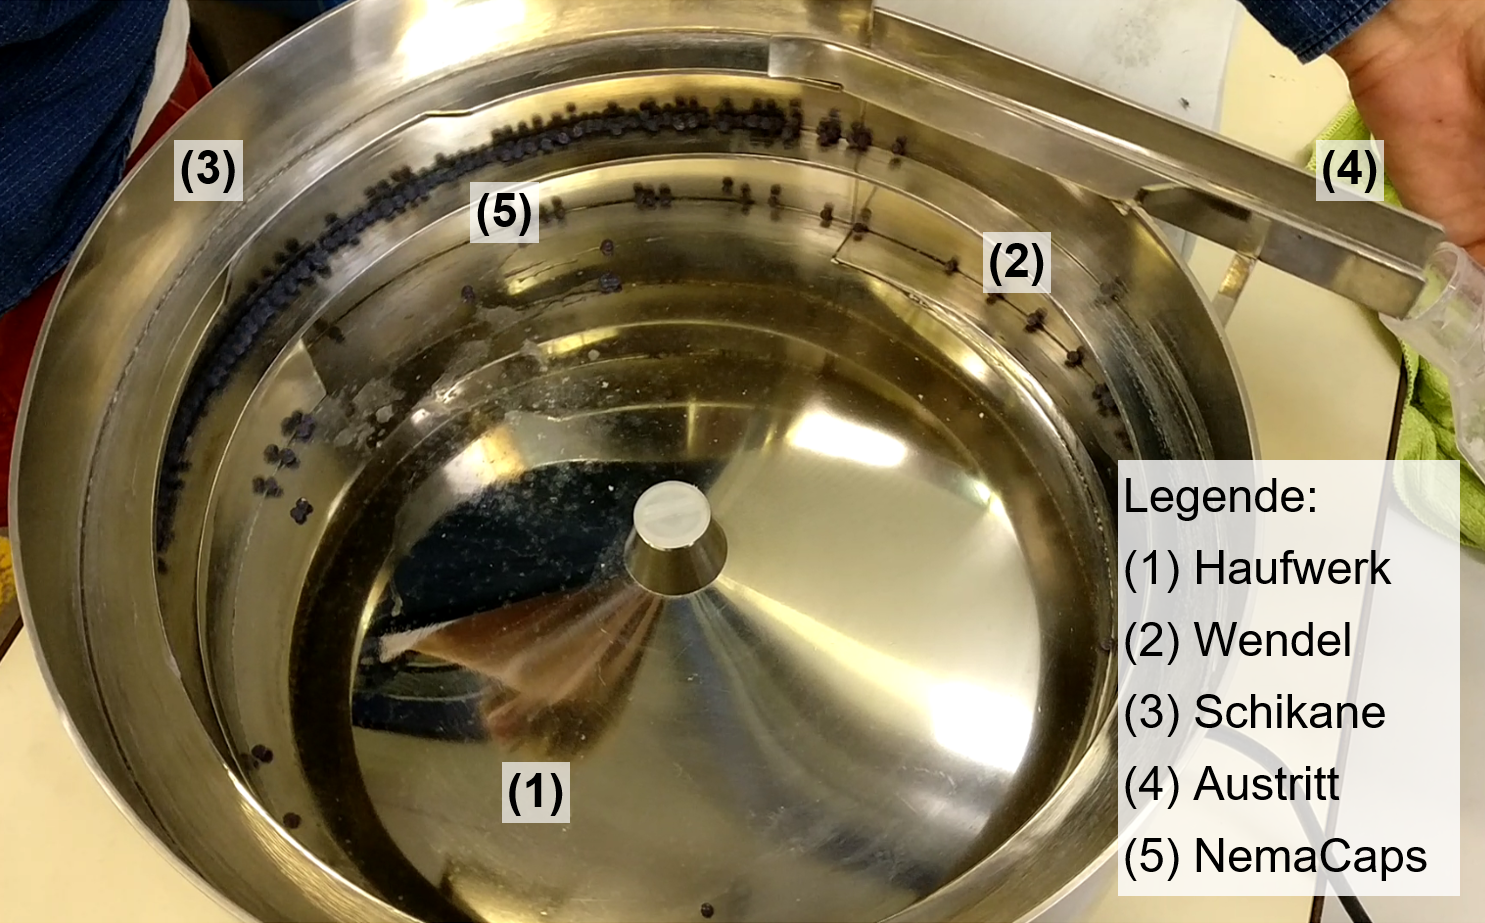
\includegraphics[width=1\textwidth]{Illustrationen/5-Konzept/wendelfoerderer.PNG}
	\caption{Praktische Tests am Wendelförderer der Hochschule}
	\label{fig:wendelfoerderer}
\end{figure}
\textbf{Erkenntnisse}
\newline
Folgende Erkenntnisse lieferten die Versuche:
\begin{itemize}
	\item Eine Förderung von NemaCaps mit einem Wendelförderer ist möglich. Die NemaCaps eignen sich als Fördergut und werden mit einer hohen Zuverlässigkeit gefördert.
	
	\item Die Schikane erfüllt ihre Funktion nicht. Dies ist allein auf die Tatsache zurückzuführen, dass der verwendete  Wendelförderer für gezuckerte Mandeln dimensioniert wurde. Eine Anpassung der Schikanen auf NemaCaps ist technisch machbar und ist kein Hindernis.
	
	\item Die Umsetzung der Funktionen NemaCaps vereinzeln und fördern mit einem Wendelförderer ist aus rein technischer Sicht realisierbar.
\end{itemize} 
\newpage
\textbf{Rotierende Lochmaske}
\newline
\begin{wrapfigure}[26]{r}{10cm}
	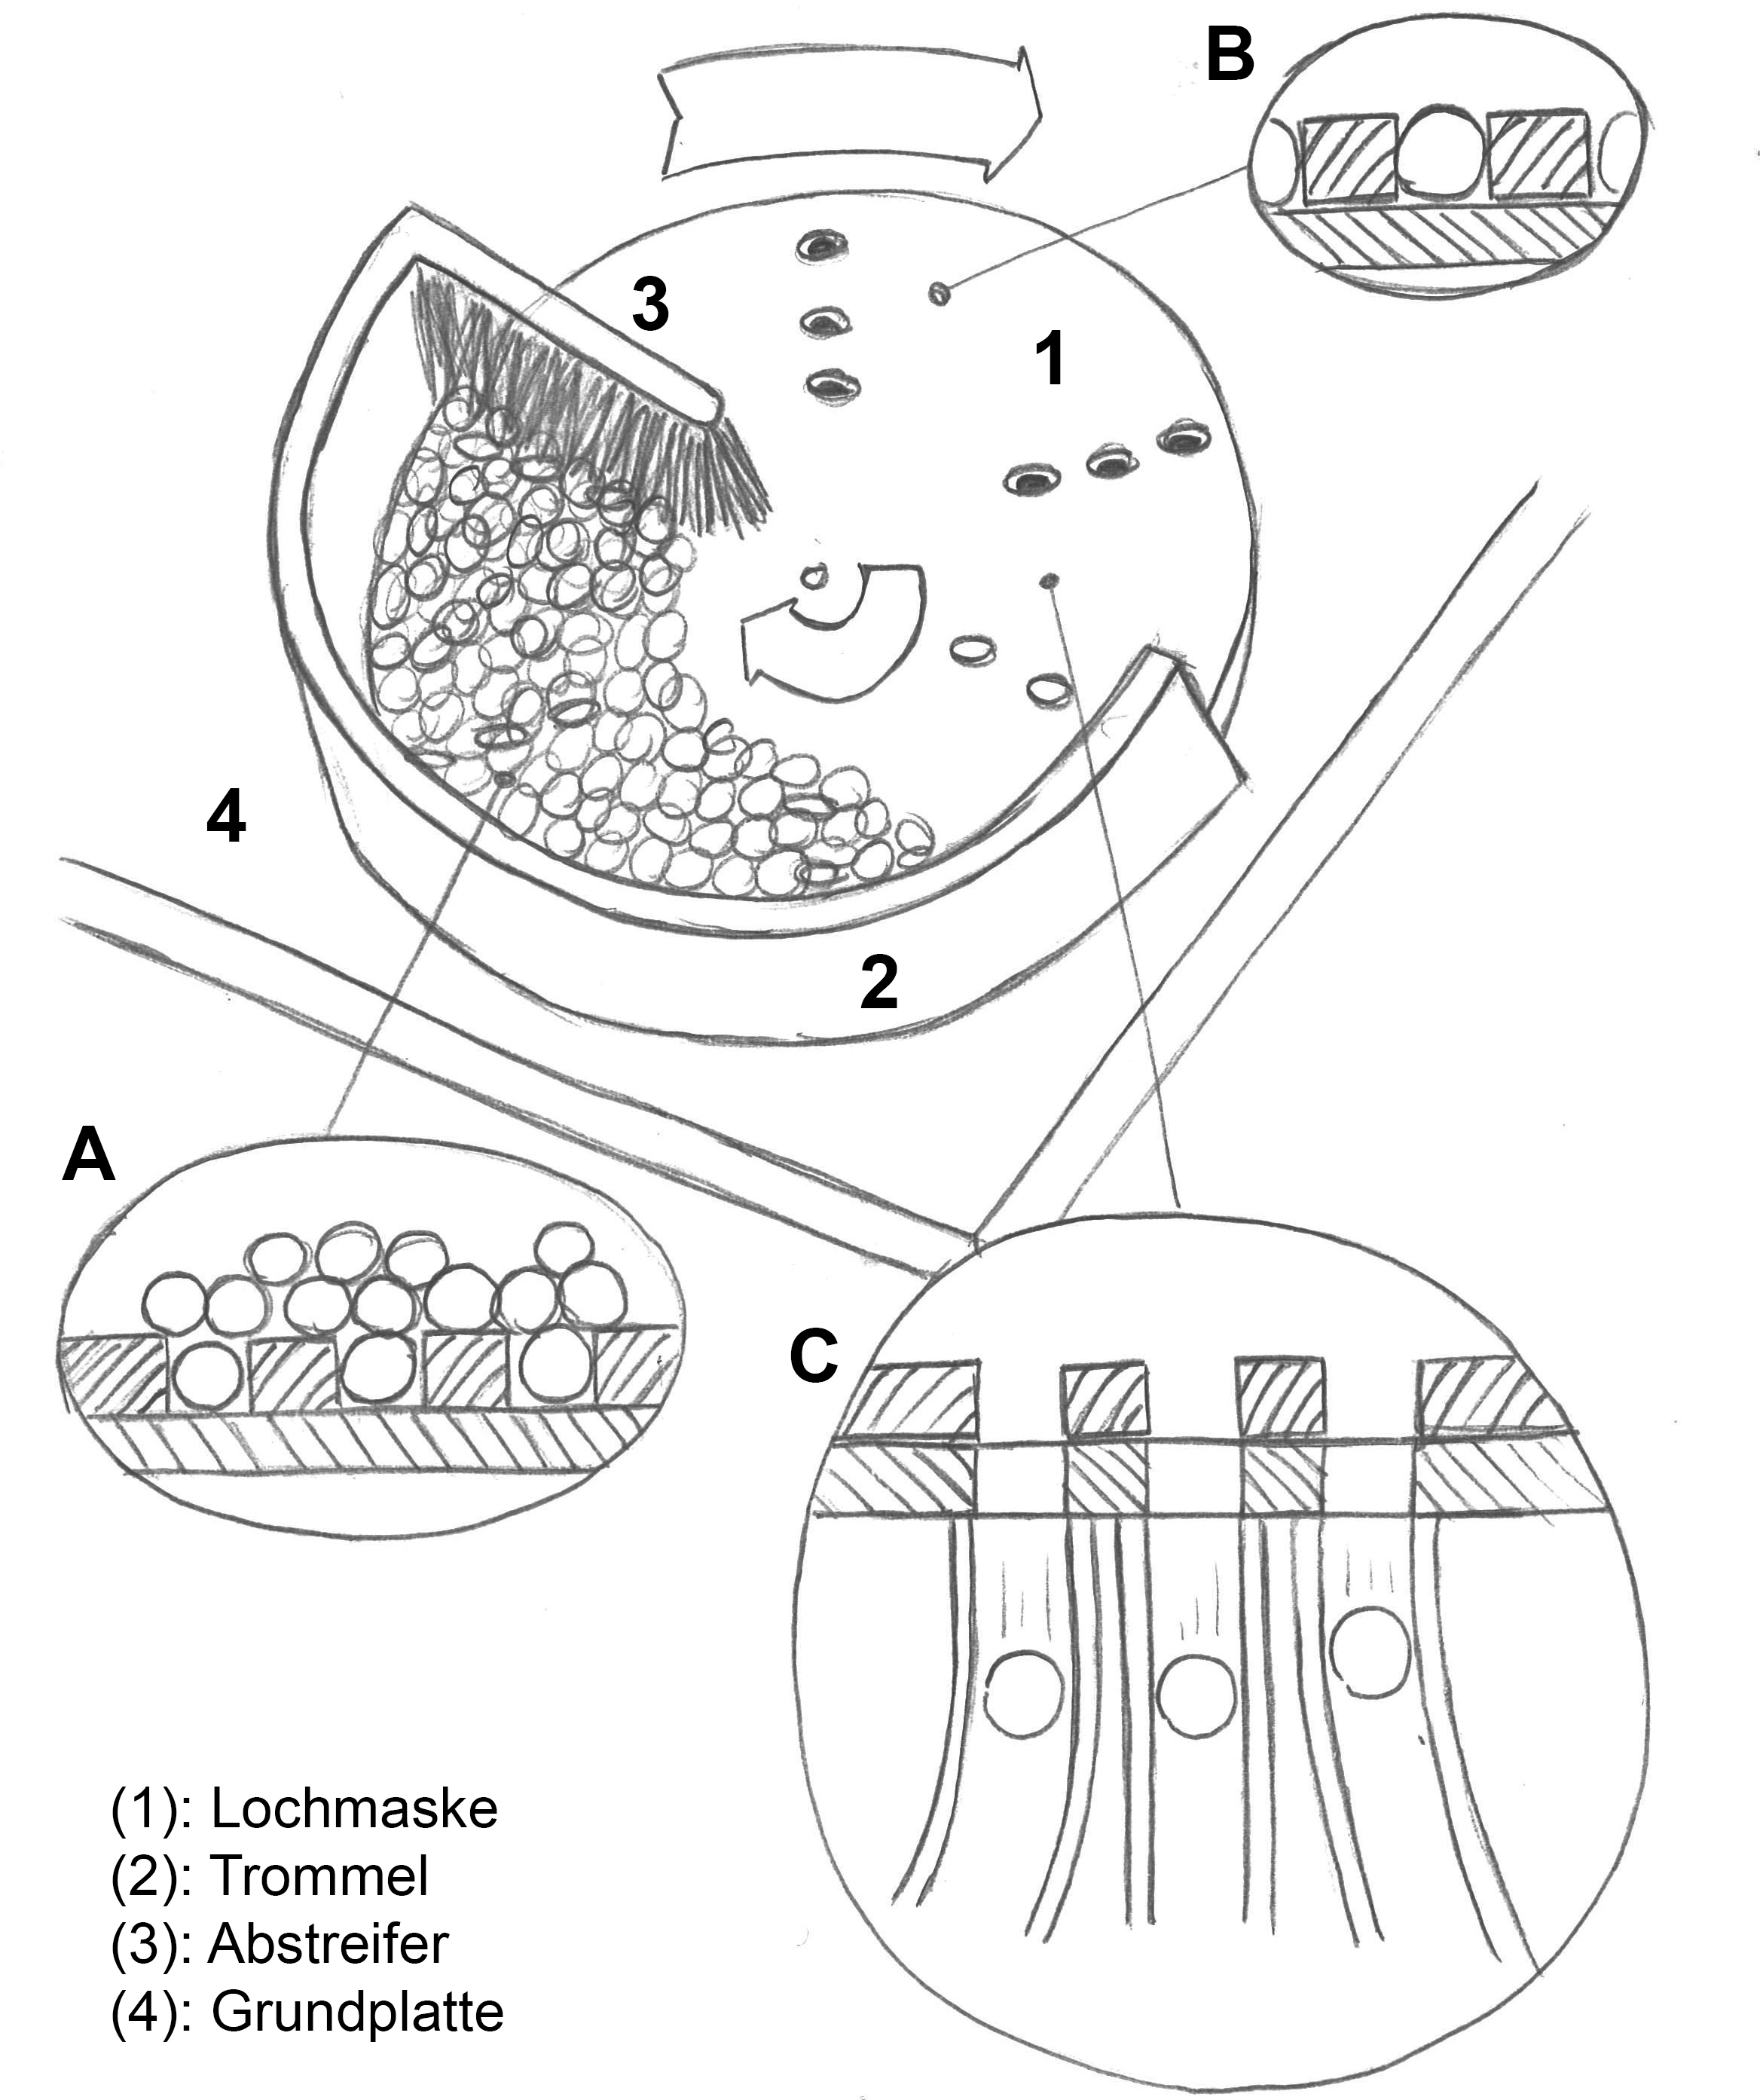
\includegraphics[scale=0.52]{Illustrationen/5-Konzept/schema_vereinzelung.jpg}
	\caption{Vereinzelung durch rotierende Lochmaske}
	\label{fig:schema_vereinzelung}
\end{wrapfigure}
Ein weiteres Konzept ist die Vereinzelung durch eine rotierende Lochmaske. Dabei werden die NemaCaps in einen Behälter gefüllt (Punkt 2 in Abbildung \ref{fig:schema_vereinzelung}). Im Behälter befindet sich eine rotierend gelagerte Scheibe mit Löchern (Lochmaske, 1). Die Löcher sind so gross, dass gerade ein NemaCap darin Platz hat. Durch die Rotation der Lochmaske fallen nun NemaCaps in die Maske (Detail A) und werden zu Detail B transportiert. Ein Abstreifer (hier in Form einer Bürste) sorgt dafür, dass überschüssige NemaCaps zurückgehalten werden. In der Grundplatte (4) sind Löcher vorgesehen, sodass bei Detail C die NemaCaps in Schläuche fallen. Idealerweise wird dieser Aufbau schief gelagert. 
\newline
\newline
Dieses Konzept wird von der Firma Kofatec GmbH für die Vereinzelung von Pfefferkörner eingesetzt. Dabei ist das Design des Funktionsnachweises stark am Funktionsmuster der Firma Kofatec GmbH angelehnt. Das Funktionsmuster wird mittels Lasermaschine aus MDF hergestellt. Auch wird die Lochmaske für den Funktionsnachweis von Hand betrieben.
\newline
Am 21.3.2017 wurde am umgesetzten Funktionsmuster der Funktionsnachweis erbracht. Durch zielgerichtetes Ausprobieren von verschiedenen Durchmesser der Löcher wurde die Lochmaske für die NemaCaps ausgelegt. Dann wurde mittels manuellem Rotieren die Vereinzelung überprüft.
\newline
\newline
Folgende Erkenntnisse lieferten die Versuche:
\begin{itemize}
	\item Die Lochmaske nimmt zuverlässig NemaCaps auf. Auch ein Transport zur Auslösung (Detail C in \ref{fig:schema_vereinzelung}) verläuft problemlos.
	
	\item Die Abstreifung von NemaCaps funktioniert. Kritisch ist dabei die Wahl des Abstreifers. Verwendet man zu scharfkantige Gegenstände kann es passieren, dass ein NemaCap verschnitten wird. Weiter wurde erkannt, dass NemaCaps heikel auf Scherbeanspruchungen reagieren. Dies Eigenschaft ist nicht zu unterschätzen.
		
	\item Die Zuverlässigkeit der Auslösung am Punkt C ist durchschnittlich. Dies wird damit erklärt, dass nicht frische NemaCaps verwendet wurden. Dadurch hat sich das hygroskope Pulver in Wasser gewandelt und so die Adhäsion der NemaCaps erhöht. Dadurch blieben geschätzte 50 Prozent der NemaCaps an der Lochmaske hängen. Auch ist ein holzfaserbasiertes Material für die Lochmaske ungeeignet. Die rauhe Oberfläche der Bohrung bietet so mehr Haftung.
	
	\item Durch leichtes Antippen der Grundplatte oder einem Luftstoss konnten alle NemaCaps ausgelöst werden. Dies zeigt, dass durch Abhilfemassnahmen durchaus eine höhere Zuverlässigkeit erreicht wird.
	
	\item Die Umsetzung von diesem Lösungsansatz ist nur realistisch, wenn klare Abhilfemassnahmen und Verbesserungen der Lochmaske zur Steigerung der Zuverlässigkeit definiert werden. 
\end{itemize} 
\textbf{Bild des Funktionstests?}

\subsubsection{NemaCaps setzen}
Ein Lösungsansatz der Teilfunktion "NemaCaps setzen" basiert auf der Idee zuerst ein Loch auszuheben oder zu verdrängen und dann ein NemaCap ins Loch fallen zu lassen. Ähnlich ist eine andere Idee, welche mit einer spitzen Zange das Loch verdrängt wird, sich die Zange in der Erde öffnet und so ein NemaCap platziert.
\newline
Um die Umsetzbarkeit dieser Ideen zu überprüfen, werden zwei Versuche durchgeführt:
\begin{itemize}
	\item \textbf{A) Ermittlung der Verdrängkraft:} Mit einer konventionellen Setzhilfe aus dem Gartenbau werden praktische Tests durchgeführt. Dabei wird ein Topf mit dem vorgegebenen Gartenhumus von Ricoter befüllt und leicht angepresst. Nun wird die maximale Einsetztiefe an der Setzhilfe markiert und schrittweise mit Gewicht (Masse m in Abbildung \ref{fig:skizze_setzversuch}) beschwert. Sobald die Markierung den Gartenhumus berührt, wird die Setzhilfe inklusive Masse m gewogen und durch die Multiplikation mit der Erdbeschleunigung die benötigte Verdrängkraft ermittelt.
	
	\item \textbf{B) NemaCap mittels Zange setzen:} Der identische Versuch wird mit der genannten Zange durchgeführt. Zusätzlich wird in die geschlossene Zange ein NemaCap gegeben. Bei Erreichung der Setztiefe wird die Zange geöffnet und das NemaCap platziert. Realisiert wird die Zange aus gelasertem MDF.
\end{itemize} 

\begin{figure}[H]
	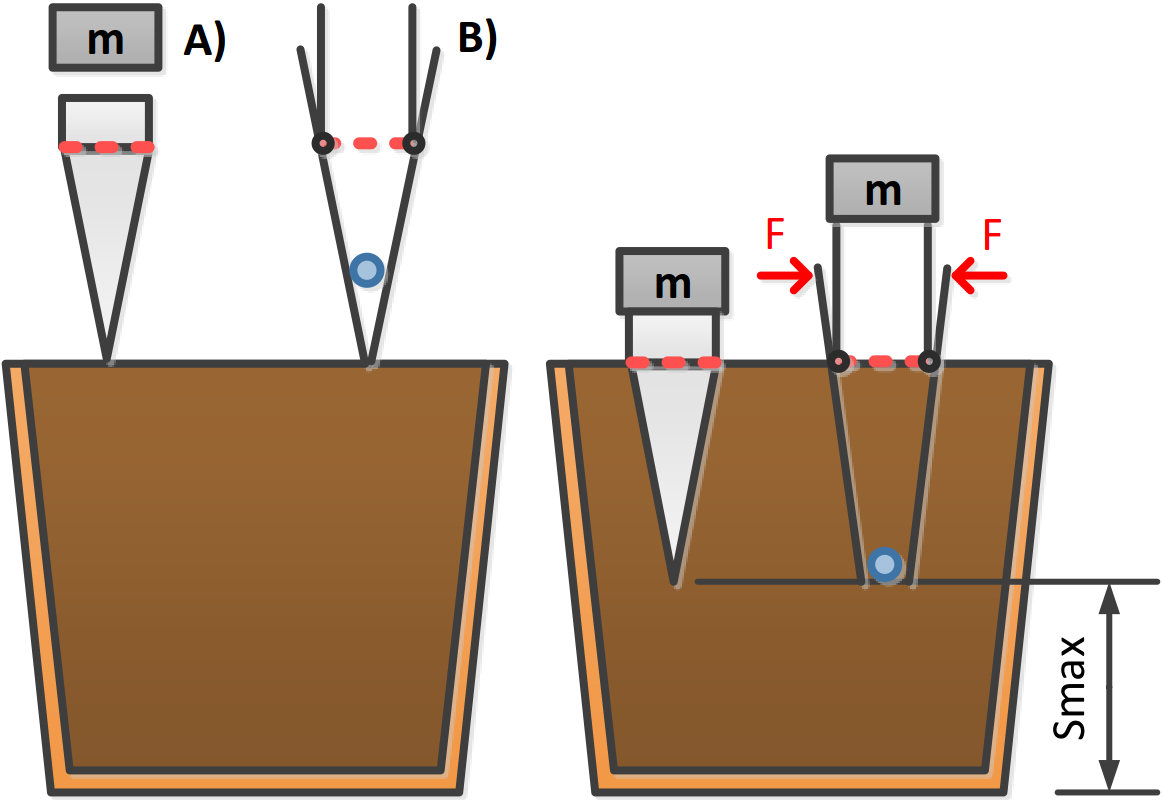
\includegraphics[width=1\textwidth]{Illustrationen/5-Konzept/skizze_stechversuch.PNG}
	\caption{Versuchsaufbau zur Ermittlung der Verdrängkraft}
	\label{fig:skizze_setzversuch}
\end{figure}

\textbf{Erkenntnisse}
\newline
Folgende Erkenntnisse lieferten die Versuche:
\begin{itemize}
	\item Mit der konventionellen Setzhilfe kann mit geringem Aufwand das erforderliche Setzloch verdrängt werden. Auch bei erschwerten Umständen wie komprimiertem Gartenhumus oder kleinerem Gehölz im Humus konnte ein Setzloch verdrängt werden. Über mehrere Versuche wurden folgende Werte ermittelt:
	\begin{tabular}{|l|c|c|}
		\hline 
		& kleinster Topf (D=90mm) & grösster Topf (D=140mm) \\ 
		\hline 
		geforderte Setztiefe [mm] & 40 & 64 \\ 
		\hline 
		benötigte Masse [kg] & 0.15 & 0.6 \\ 
		\hline 
		Verdrängungskraft[N] & 1.5  & 6.0  \\ 
		\hline 
	\end{tabular} 
	
	\item Der gegebene Gartenhumus von Ricoter besitzt gute Eigenschaften für diese Anwendung. Nach der Verdrängung behält das Setzloch seine Form bei, sodass die Bedingungen für das Einsetzen des NemaCaps gegeben sind. Dabei ist darauf zu achten, dass stets frischer Gratenhumus verwendet wird.
	
	\item Tests mit der Zange ergaben, dass eine Verdrängung der Erde mit dem identischen Kraftaufwand machbar ist. In der erforderlichen Setztiefe angekommen, benötigt es einen erhöhten Kraftaufwand, um die Zange zu öffnen und das NemaCap zu platzieren. Wie eine Streckenlast wirkt die zu verdrängende Erde der Bewegung entgegen und erschwert die Öffnung. Diese Teillösung wird als nicht umsetzbar eingeschätzt.
\end{itemize} 

\subsubsection{Setzmechanismus konfigurieren}
Die automatische Konfuguration des Setzmechanismus ist als Wunschanforderung im Pflichtenheft formuliert. Gemeint ist dabei die automatische Verstellung der Radien der Einsatzlokalität. Ein ausgearbeiteter Lösungsansatz basiert auf zwei Kulissen, welche drei dorne halten. Über die Rotation der einen Kulisse kann so der Dorn radial verstellt werden. Umgesetzt werden die Kulissen anhand ausgelaserten Scheiben (siehe Abbildung \textbf{XY}). Dabei wird dieses Funktionsmuster manuell von Hand betrieben.
\newline
\textbf{Bild des umgesetzten Funktionsmusters}
\newline
Folgende Erkenntnisse lieferten das Funktionsmuster:
\begin{itemize}
	\item Die manuelle Verstellung des Radius mittels kulisse ist möglich. Durch eine Drehbewegung werden die Dorne synchron verstellt.
	
	\item Aus der Geometrie der Kulissen wird erkennbar, dass die maximale Rotation 45° beträgt. Dies muss bei einer allfälligen Evaluation des Antriebes berücksichtigt werden.
	
	\item Am Rand der Kulisse nimmt der Kraftaufwand für eine Verstellung deutlich zu. Auch kommt es vor, dass die Kulisse an Rand kaum in Bewegung gerät. Dies ist damit erklärbar, dass an diesem Punkt die Wirkungslinien der Kulissen normal zueinander stehen und so kein Moment auf die äussere Kulisse wirken kann. Bei einer allfälligen Umsetzung müssen die Wirkungslinien der Kulissen möglichst parallel verlaufen. 
\end{itemize} 
\subsubsection{Topferkennung}